\chapter{Konzeptentwicklung}

Ziel des Konzeptes ist es eine möglichst automatisierte Erstellung digitaler Zwillinge ohne manuelle Interaktion bereitzustellen. Dies bringt verschiedene Vorteile mit sich, vor allem aber, können so dynamisch neue Zwillinge für neue Geräte generiert werden. Dabei ist es auch die Aufgabe bereits bestehende Geräte, sich im Falle einer Netzwerkpartition wieder mit ihrem entsprechenden Zwilling zu verbinden.\\
Dabei muss berücksichtigt werden, dass verschiedene Services bei dem Erstellen und dem Aufrechterhalten der Verbindung genutzt werden.

Eine wichtige Komponente stellt dabei die \textbf{Device Registry} dar. IBM definiert die Funktion einer Device Registry folgendermaßen:

\begin{definition}[Device Registry]
    \enquote{The Device Registry is the most important part of any IoT solution. With the registry, you can manage your device types and manage, maintain, and monitor the devices that you register.}\autocite{ibm_dr}\label{def:device_registry}
\end{definition}

Aus dieser Definition lassen sich mehrere wichtige Eigenschaften entnehmen. Zum einen stellt eine Device Registry einen zentralen Bestandteil dar. Dort liegt die Verwaltung der verscheidenen Geräte, welche alle entweder eigenständig oder miteinander kombiniert zur Erstellung digitaler Zwillinge genutzt werden können. Es geht auch hervor, dass die Art des Gerätes keine Rolle spielt - es können sogar verschiedene Typen verwaltet werden. Gleichzeitig dient es auch als zentrale Anlaufstelle, um die Authentizität von Geräten zu verifizieren. So muss eine Device Registry auch Mechanismen implementieren, die es ermöglichen tausende Geräte zu identifiezieren und zu verwalten.

Alle Bestandteile einer Device-Regisry lassen sich auf Abbildung \vref{fig:device_registry} erkennen. Für jeden Anwendungsfall eine eigene Device Registry aufzusetzen, Ressourcen für den Betrieb zu allokieren und zu warten gestaltet sich als unpraktisch. 
Deswegen sind die Registries verschiedener Anbieter \footnotetext{Google IoT Core, IBM, Eclipse Hono} mit einem Namespace System ausgestattet, sodass mehrere Nutzer abgetrennt voneinander innerhalb derselben Registry verwendet werden können.

\begin{figure}
    \centering
    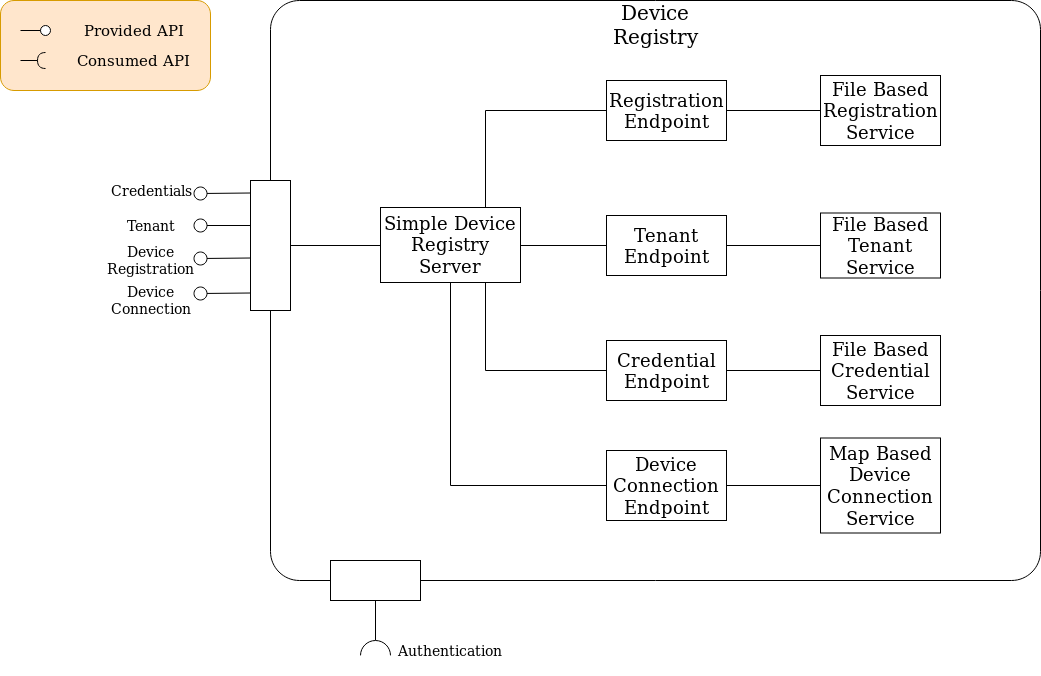
\includegraphics[width=0.75\linewidth]{img/device-registry.png}
    \caption[Bestandteile einer Device Registry]{Beispielhafter Aufbau einer Device Registry am Beispiel von Eclipse Hono. Quelle: \url{https://www.eclipse.org/hono/docs/architecture/component-view/device-registry.png}}
    \label{fig:device_registry}
\end{figure}

Inhärent bedeutet das, dass das Authentifizierungs- und Authorisierungssystem dieses Scoping unterstützen muss. Somit benötigt die Umsetzung der Authentifizierung eine genauere Begutachtung.

\section{Authentifizierung und Authorisierung von IoT Geräten}
\label{sec:auth}

Die Authentifizeriung von Geräten im IoT Bereich stellt eine Herausforderung dar. So ist es unpraktisch, für jedes Gerät eigene Zugangsdaten zu generieren und auf dem Gerät zu hinterlegen, damit es sich bei der Device Registry identifizieren kann. Auch birgt es ein Sicherheitsproblem, sollten sich Geräte eigenständig in der Device Registry registrieren können, ohne vorher Beweisen zu können, dass sie Zugriff auf einen bestimmten Namespace haben. \\
Es gilt also eine Alternative zu finden, welche es ermöglicht Geräte im großen Stil mit Zugangsdaten auszustatten, welche allerdings nicht Geräteindividuell angepasst werden müssen.\\
Um das manuelle Hinterlegen geräteindividueller Zugangsdaten zu vermeiden müssen Alternativen untersucht werden, welche eine Vorauthentifizierung ermöglichen. 

Eigentliches Ziel der Authentifizierung ist der Nachweis einer behaupteten Eigenschaft einer Entität. Bricht man das Problem der Geräteauthentifizierung auf diesen Sachverhalt herunter, lässt sich erkennen, dass viele Konzepte der Krypthographie ähnliche oder gleiche Probleme bearbeiten. Ziel innerhalb der Kryptogrpahie ist unter anderen der Aufbau eines sicheren Kommunikationskanals zwischen verschiedenen Parteien. Umformuliert lässt sich das Problem folgendermassen darstellen:

\begin{problem}[Authentifizierung]
    Partei $A$ behauptet gegenüber Partei $B$, vertrauenswürdig zu sein.
\end{problem}

Dank dieser Transformation können nun Lösungen und Hilfsmmittel aus der Krypthographie zur Bearbeitung des Authentifizierungsproblems herangezogen werden.

Grundsätzlich gilt es innerhalb der Kryptographie zwei Formen der Verschlüsselung zu unterscheiden:

\begin{enumerate}
    \item Die \textbf{symmetrische Verschlüsselung}, welche darauf beruht, dass zwei Schlüssel ausgetauscht werden, die im Anschluss genutzt werden können, um eine sichere Kommunikation aufrecht zu erhalten.
    \item  Die \textbf{asymmetrische Verschlüsselung}, die mithilfe eines öffentlichen und eines privaten Schlüssels eine sichere Kommunikation aufbaut und aufrecht erhält.
\end{enumerate}

Ein bekannter Nachteil symmetrischer Verschlüsselungsmethoden, ist der Schlüsselaustausch und das Sicherstellen einer sicheren Kommunikation zwischen einer wachsenden Anzahl an Teilnehmern. Somit wäre eine symmetrische Art der Verschlüsselung suboptimal für einen Anwendungsfall bei digitalen Zwillingen. \marginpar{Warum?}

Alternativ bieten sich dann noch Möglichkeiten asymmetrischer Verschlüsselungsarten an. Ein Vorteil dieser Art ist es, dass ein Schlüssel austausch sehr einfach erreicht werden kann, da der Aufbau der Verbindung auf Basis eines öffentlichen Schlüssels basiert. Nachteil dieser Methode ist es allerdings, dass der Verbindungsaufbau und die Geschwindigkeit der Verschlüsselung sehr langsam ist. Im speziellen wenn größere Datenmengen verschlüsselt werden müssen sind symmetrische Verschlüsselungen deutlich schneller. Außerdem stellen symmetrische Chiffren ein höheres Sicherheitsniveau zur Verfügung.

\subsection{Pre-Authentication via Zertifikat}
\label{sec:certificate}

Um soviele Vorteile wie möglich bei gleichzeitig so wenig Nachteilen wie nötig zu erhalten, ist es am sinnvollsten beide Ansätze miteinander zu kombinieren. Diese Idee wird bereits in der Internetkommunikation verwendet. Dabei wird mithilfe eines asymmetrischen Schlüsselpaars ein sichere Kanal zur Kommunikation für einen symmetrischen Schlüsselaustausch und die anschließende Verschlüsselung aufgebaut. \\
Durch den Einsatz eines Zertifikates können die beschriebenen Vorteile erreicht werden.

\subsubsection*{Aufbau eines Zertifikates}

Durch \citeauthor{RFC3280} wurde ein Standard definiert, welcher zur Authentifizierung mit Zertifikaten genutzt werden soll. Dabei handelt es sich um den X.509 Standard. In \vref{fig:cert_structure} wird die grundlegende Struktur eines Zertifikates beschrieben. Die für den Anwendungsfall wichtigsten Informationen lassen sich dabei in der Struktur eines \texttt{TBSCertificate} finden. Dazu zählen die Informationen über den Herausgeber (Issuer) und den Zweck (Subject) des Zertifikats. \autocite{RFC3280}

\begin{definition}[Subject]
    Where it is non-empty, the subject field MUST contain an X.500 distinguished name (DN).  The DN MUST be unique for each subject entity certified by the one CA as defined by the issuer name field. \autocite[Kapitel~4.1.2.6]{RFC3280}
\end{definition}

\begin{verbatim}
Certificate  ::=  SEQUENCE  {
    tbsCertificate       TBSCertificate,
    signatureAlgorithm   AlgorithmIdentifier,
    signatureValue       BIT STRING  }
TBSCertificate  ::=  SEQUENCE  {
    version         [0]  EXPLICIT Version DEFAULT v1,
    serialNumber         CertificateSerialNumber,
    signature            AlgorithmIdentifier,
    issuer               Name,
    validity             Validity,
    subject              Name,
    subjectPublicKeyInfo SubjectPublicKeyInfo,
    issuerUniqueID  [1]  IMPLICIT UniqueIdentifier OPTIONAL,
                            -- If present, version MUST be v2 or v3
    subjectUniqueID [2]  IMPLICIT UniqueIdentifier OPTIONAL,
                            -- If present, version MUST be v2 or v3
    extensions      [3]  EXPLICIT Extensions OPTIONAL
                            -- If present, version MUST be v3
    }
Version  ::=  INTEGER  {  v1(0), v2(1), v3(2)  }
CertificateSerialNumber  ::=  INTEGER
Validity ::= SEQUENCE {
    notBefore      Time,
    notAfter       Time }
Time ::= CHOICE {
    utcTime        UTCTime,
    generalTime    GeneralizedTime }
UniqueIdentifier  ::=  BIT STRING
SubjectPublicKeyInfo  ::=  SEQUENCE  {
    algorithm            AlgorithmIdentifier,
    subjectPublicKey     BIT STRING  }
\end{verbatim}
\label{fig:cert_structure}
\begin{center}
    \small \fullcite{RFC3280}
\end{center}

Um massenhaft Geräte zu authentifizieren kann während der Erstellung eines Namespaces/Tenants innerhalb der Device Registry ein Zertifikat inklusive korrespondierendem \textit{private Key} hinterlegt werden, dess Zweck darin besteht, als Identifikator für Geäte zu dienen. Bei einem Verbindungsversuch kann dann seitens des Authentifizierungsservice überprüft werden, ob das mitgesendete Zertifikat für den angefragten Tenant gültig ist. Anschließend können dann über dieses \enquote{sicheren Kanal} gerätespezifische Zugangsdaten generiert oder ausgetauscht werden.

Mithilfe dieser Gerätezugangsdaten kann eine zukünftige Identifikation der Geräte durchgeführt werden.

\begin{figure}[ht]
    \centering
    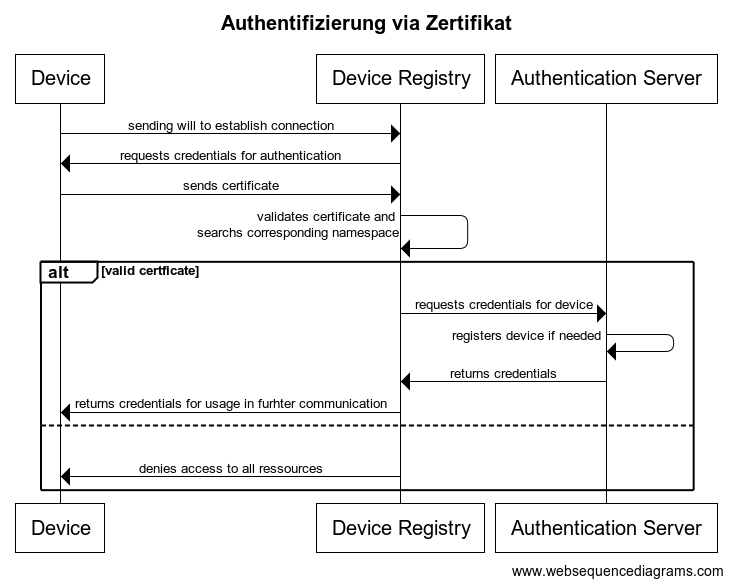
\includegraphics[width=1.0\linewidth]{img/device_authentication.png}
    \caption[Ablauf der Authentifizierung via Zertifikat]{Ablauf der Authentifizeriung eines Gerätes via Zertifikat.\\ Quelle: Eigene Darstellung}
    \label{fig:certificate}
\end{figure}

In Abbildung \vref{fig:certificate} ist zu erkennen, wie der Ablauf einer solchen Authentifizierung sein kann.

\subsection{Direkter Einsatz der Device Zugangsdaten}
\label{sec:credentials}

Werden die Zugangsdaten direkt auf dem Gerät hinterlegt, entsteht das oben beschriebene Problem. Das vorherige generieren dieser Zugansdaten bringt verschiedene Probleme mit sich, wenn die Geräte, die im späteren System eingesetzt werden, nicht final bekannt sind. Zudem muss außerdem noch da Problem gelöst werden, wie Zugangsdaten auf ein Gerät gelangen können.

Dieser Nachteil kann allerdins ignoriert werden, sollten es eigene Geräte sein, oder falls sich alle Geräte vor einem produktiven Einsatz in einer \enquote{Einrichtungsphase} befinden. Mithilfe dieser Methode könnte die Aufgabe der Zertifikaterstellung und -validierung von der Device Registry entfernt werden, was ein insgesamt klareres System erzeugt.

\subsection{Vergleich beider Authentifizierungsvarianten}

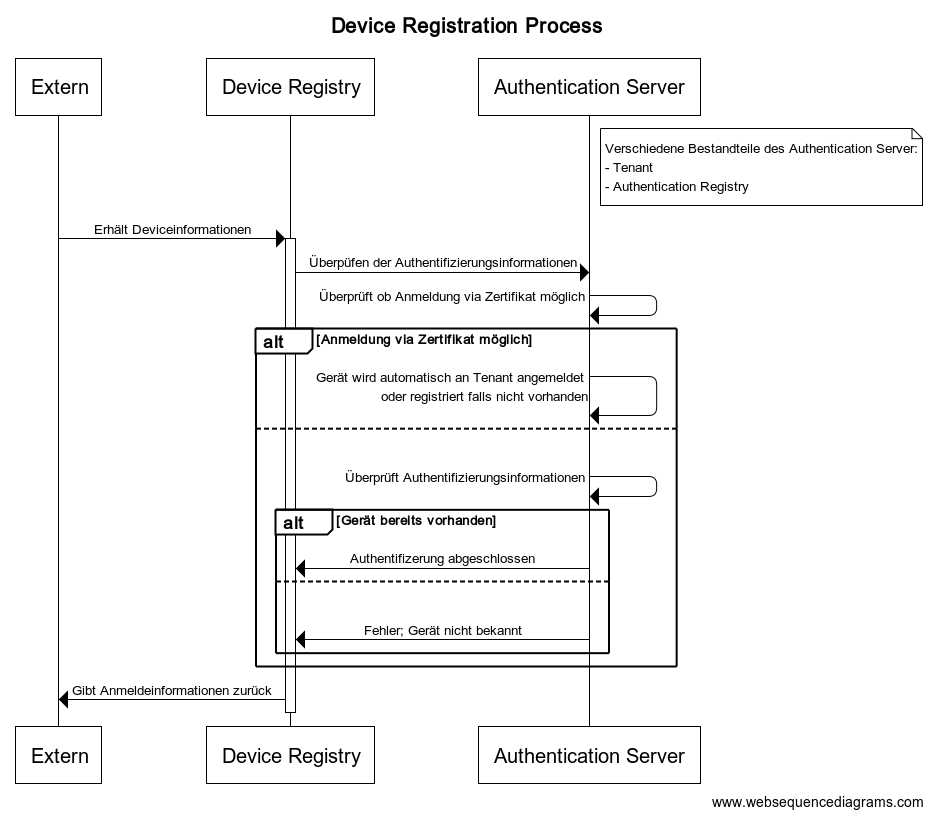
\includegraphics[width=0.8\linewidth]{img/device_registration.png}

\section{Sicherstellen der Device Connectivity in der Device Registry}

Der Device Registry fällt ebenfalls die Aufgabe zu, sicherzustellen, dass eine Vielzahl verschiedener Kommunikationsprotokolle unterstützt wird, damit ein Verbindungsaufbau mit einer Vielzahl von Geräten möglich ist. Im folgenden werden verschiedene Kommunikationsprotokolle vorgestellt, sowie kurz deren jeweilige Vor- und Nachteile beleuchtet. Im nächsten Schritt wird die Wahl eines asynchronen, internen Kommunikationsmittels beschrieben.

\subsection{MQTT}
Bei dem \ac{MQTT} handelt es sich um ein sehr populäres Kommunikationsprotokoll, das in den letzten Jahren immer mehr an Popularität gewonnen hat. Das \ac{MQTT} Protokoll definiert folgende Bestandteile:

\begin{definition}[MQTT]
    MQTT\autocite{standard2014mqtt} is a Client Server publish/subscribe messaging transport protocol. [...]These characteristics make it ideal for use in many situations, including constrained environments such as for communication in Machine to Machine (M2M) and Internet of Things (IoT) [...].

    The protocol runs over TCP/IP [...]. Its features include:

    \begin{itemize}
        \item Use of the publish/subscribe message pattern which provides one-to-many message distribution and decoupling of applications.
        \item A messaging transport that is agnostic to the content of the payload.
        \item A small transport overhead and protocol exchanges minimized to reduce network traffic.
        \item A mechanism to notify interested parties when an abnormal disconnection occurs.
    \end{itemize}
\end{definition}

Bei der Nutzung des MQTT-Protokolls werden zwei Bestandteile benötigt. Zum einen der \textbf{MQTT-Client}, welcher auf den Endgeräten genutzt wird und eine Kommunikation mit dem \textbf{MQTT-Broker} aufbaut.\\ Kernaufgabe des Brokers ist es dabei, die verschiedenen Topics inklusive den zugehörigen Subscribern und Zustellungsvorgaben zu verwalten. Um eine möglichst hohe Ausfallsicherheit zu gewährleisten können mehrere Broker bereitgestellt werden. Mithilfe entsprechender Konfiguration ist es möglich, im Falle eines Ausfalls auf andere Broker auszuweichen, ohne einen Verbindungs- oder Kommunikationsverlaust zu erleiden.

Wird das \ac{MQTT} Protokoll innerhalb einer Device Registry genutzt wird nicht der gesamte Funktionsumfang eines Brokers benötigt. Wichtig ist dabei nur, dass Nachrichten, die dem \ac{MQTT} Standard folgen, von der Registry korrekt interpretiert werden können.\\
Dabei gilt es auch zu unterscheiden, ob es sich um unidirektionale oder bidirektionale Kommunikation handelt. 

\subsection*{Unidirektionale Kommunikation}
Ziel dieser Form der Kommunikation innerhalb dieses spezifischen Anwendungsfalls ist das Senden der Telemetrieinformationen von dem Gerät zu der Device-Regitry, welche im diesem Fall die Rolle des Brokers einnimmt.

Dabei werden hauptsächlich \textit{Telemetrieinformationen} des Gerätes an die Device Registry weitergegeben. 

\begin{figure}[h]
    \centering
    \begin{tikzpicture}[node distance=2cm]
        \node (dev1) [io] {Endgerät};
        \node (dev2) [process, right of=dev1, xshift=6.5cm] {MQTT-Adapter der Device Registry};
        \draw [arrow] (dev1) -- node[anchor=south] {Telemetry} (dev2);
        \draw [thick, dashed] (dev2) -- (13,0);
    \end{tikzpicture}
    \caption[Unidirektionale Kommunikation]{Unidirektionale Kommunikation zwischen Endgerät und Device Registry.\\Quelle: Eigene Darstellung}
\end{figure}

\subsection*{Bidirektionale Kommunikation}
Im Gegensatz zu der unidirektionalen Kommunikation steht bei der bidirektionalen Kommunikation die Informationsübermittlung zwischen beiden Komponenten im Vordergrund. So werden nicht nur Telemetrieinformationen des Endgerätes an die Device-Registry übermittelt, sondern auch Befehle o.ä. an das Endgerät.

\begin{figure}[h]
    \centering
    \begin{tikzpicture}[node distance=2cm]
        \node (dev1) [io] {Endgerät};
        \node (dev2) [process, right of=dev1, xshift=6.5cm] {MQTT-Adapter der Device Registry};
        \draw [arrow] (dev1) -- node[anchor=south] {Telemetry} (dev2);
        \draw [arrow] (dev2) -- node[anchor=north] {Kommandos, etc.} (dev1);
        \draw [thick, dashed] (dev2) -- (13,0);
    \end{tikzpicture}
    \caption[Bidirektionale Kommunikation]{Bidirektionale Kommunikation zwischen Endgerät und Device Registry.\\Quelle: Eigene Darstellung}
\end{figure}

Eine Besonderheit der bidirektionalen Kommunikation mittels \ac{MQTT} stellt das fehlende Request-Response Pattern dar. Bei anderen Protokollen (wie z.B. HTTP) ist in das Protokoll ein Mechanismus eingebaut, um auf die Anfrage eines Clients eine Antwort an nur diesen Client zurückzugeben. Dieses Konzept wurde innerhalb der MQTT Spezifikation nicht umgesetzt. Stattdessen kann dort mittels klar definierten Topic Strukturen ein Request-Reponse Pattern integriert werden.
\pagebreak
\begin{example}[Request-Response innerhalb von MQTT] Eine examplarische Methode zur Integration eines Request-Response Pattern kann folgender Abbildung entnommen werden. Dabei ist zu erkennen, dass das Zeil mithilfe einer bestimmten Topicstruktur erreicht wird. Diese Topicstrukturen können innerhalb von MQTT nicht erzwungen werden, sodass nicht sichergestellt ist, dass dieses Konzept zuverlässig funktionert.

    \begin{figure}[h]
        \centering
        \begin{tikzpicture}[node distance=2cm]
            \node (dev1) [process] {Endgerät};
            \node (dr1) [process, right of=dev1, xshift=8.5cm] {MQTT-Broker};
            \node (dev2) [process, below of=dev1] {Endgerät};
            \node (dr2) [process, right of=dev2,below of=dr1, xshift=-2cm] {MQTT-Broker};

            \draw [arrow] (dev1) -- node[anchor=south] {request/<unique identifier>} (dr1);
            \draw [thick] (dev2) -- node[anchor=south] {subscribe response/<unique identifier>} (dr2);
        \end{tikzpicture}
        \caption[Request-Response Pattern innerhalb von MQTT]{Beispielhafte Umsetzung eines Request-Response Patterns innerhalb von MQTT.\\Quelle: Eigene Darstellung}
    \end{figure}
\end{example}

Zur Nutzung des \ac{MQTT} Protokolls muss eine Device Registry eine Möglichkeit bereitstellen, via MQTT mit Endgeräten zu kommunizieren. Um dieses Ziel zu erreichen kann ein Broker verwendet werden. Ein sehr populärer Vertreter eines Brokers stellt das Eclipse Mosquitto Projekt dar.\\
Gleichzeitig muss eine authentifizierte Kommunikation gewährleistet werden können. Wie in \vref{sec:auth} beschrieben, wird vorgelagert mittels eines Zertifikats sichergestellt, dass das Endgerät eindeutig identifizierbare Zugangsdaten besitzt. Diese Zugangsdaten können verwendet werden, um mithilfe eines eindeutigen Identifikators des Namespaces die \texttt{username} und \texttt{password} Informationen während der Kommunikation zu nutzen.

\subsection{AMQP}

\begin{definition}
    The \ac{AMQP} is an open internet protocol for business messaging. It defines a binary wire-level protocol that allows for the reliable exchange of business messages between two parties. AMQP has a layered architecture and the specification is organized as a set of parts that reflects that architecture. Part 1 defines the AMQP type system and encoding. Part 2 defines the AMQP transport layer, an efficient, binary, peer-to-peer protocol for transporting messages between two processes over a network. Part 3 defines the AMQP message format, with a concrete encoding. Part 4 defines how interactions can be grouped within atomic transactions. Part 5 defines the AMQP security layers.
\end{definition}

Ähnlich wie bei \ac{MQTT} gibt es innerhalb von \ac{AMQP} mehrere Akteure. Es gibt einen sogenannten \textit{Produzenten} der Nachricht, welche die zu übertragenden Informationen spezifiziert. Die Nachricht stellt dabei das Kernelement der gesamten Kommunikation dar. Diese Nachricht wird dann in einem Message Broker verarbeitet. Die Aufgaben des Message Brokers ist dabei äquivalent zu dem \ac{MQTT} Protokoll. Ein \textit{Konsument} kann sein Interesse an bestimmten Nachrichten bekunden, indem er auf sogenannte \textit{Exchanges} subscribed. Der Konsument hat somit die Möglichkeit Nachrichten, die innerhalb dieses Themas publiziert wurden anzufordern und zu verarbeiten.

\ac{AMQP} unterscheidet sich allerdigns in der Funktionsweise des Brokers von \ac{MQTT}. Innerhalb des Brokers gibt es drei Kernbestandteile:
\begin{enumerate}
    \item Die \textbf{Exchange}:\\
    Die Exchange definiert die Art der Nachrichtenübermittlung, im speziellen, ob es sich dabei um einen \textbf{Direct Exchange}, oder einen \textbf{Fanout Exchange} handelt. Der Direct Exchange stellt Nachrichten an einen einzigen Empfänger durch, wohingegen der Fanout Exchange die Nachricht an alle interessierten Queues vervielfältigt. Es gibt also zwei verschiedene Arten der Kommunikation mit einem oder wenigen Empfängern. Im Gegesnatz zu den obigen Methoden steht der sog. \textbf{Topic Exchange}. Der Topic Exchange ermöglicht es Platzhalter zu verwenden, um so nicht auf alle spezifischen Routen subscriben zu müssen.
    \item Die \textbf{Routes}:\\
    Routen stellen die Verbindung zwischen der Exchange und er Queue dar. Sie leiten Nachrichten, welche in einer Exchange zur Verfügung gestellt werden, zu den interessierten Queues weiter. Entsprechend der gewählten Art der Exchange werden entsprechende Routing Regeln angelegt. Sie dienen daher als reine Nachrichtenübermittler
    \item Die \textbf{Queues}:\\
    Queues können entweder von dem Broker oder von einem Client mit einem Identifikator versehen werden. Queues stellen einen physischen Speicher dar, welcher als Speicher für die Nachrichten dient, die mittels einer Exchange publiziert werden. Clients interagieren direkt mit der Queue, um Nachrichten zu empfangen.
\end{enumerate}

In der Abbildung \vref{fig:message_flow_amqp} ist der Zusammenhang der verschiedenen Komponenten anhand der Verarbeitung einer Nachricht visualisiert.

\begin{figure}
    \centering
    \begin{tikzpicture}[node distance=4cm]
        \node (publisher) [io] {Publisher};
        \node (exchange) [process, right of=publisher] {Exchange};
        \node (route) [process, right of=exchange] {Route};
        \node (queue) [process, below of=route] {Queue};
        \node (client) [io, below of=publisher] {Client};
    
        \draw [arrow] (publisher) -- (exchange);
        \draw [arrow] (exchange) -- (route);
        \draw [arrow] (route) -- (queue);
        \draw [arrow] (queue) -- (client);
    \end{tikzpicture}
    \caption{Verarbeitung einer Nachricht über einen \ac{AMQP} Message Broker.\\Quelle: Eigene Darstellung}
    \label{fig:message_flow_amqp}
\end{figure}

Der Nachteil eines fehlenden Request-Response Patterns von \ac{MQTT} ist dank der \textbf{Direct Exchange} direkt in \ac{AMQP} gelöst. Dies ermöglicht zusätzlich zu allen Funktionen, welche von \ac{MQTT} angeboten werden, einen erweiterten Einsatzbereich.

\subsection{LoRaWAN}
\subsection{Anforderungen an ein internes Kommunikationsmittel}

\begin{itemize}
    \item Anfragestruktur mit Pufferlösung ist wichtig, damit bei vielen Anfrage keine Verloren geht.
    \item HTTP fällt weg, da nicht pufferbar und es iwann einen timeout gibt, wenn die anfrage nicht beantwortet wird. Websockets wären eine alternative, dabei würde aber die Last massiv auf dem/den Servern liegen, was zu Problemen führen kann. eleganter wäre eine Lösung mittels eines Message Brokers. Welche kommen in Frage?
    \item MQTT sehr bekannt, oft eingesetzt, hat aber keinen Support for Req-Res pattern, was in einem Microserviceumfeld schwierigkeiten bereitet.
    \item AMQP bietet sich an, da schnell (binary Protocol), unterstützt Req-Res Pattern und ist Brokerbasiert, sodass anfragen gepuffert werden und asynchron abgearbeitet werden können.
\end{itemize}

\begin{enumerate}
    \item Architekturkonzept
    \begin{itemize}
        \item Unterscheidung zwischen einer Device-Registry und der Speicherung als DT
        \begin{itemize}
            \item Hier liegt der Übergang der Arbeit; Es müssen von Geräten in der Device Registy DTs gebildet werden, nach möglichkeit automatisiert, sodass dann Daten des Gerätes übertragen werden
        \end{itemize}
        \item Was muss eine DT-Architektur mit sich bringen, damit Definition erfüllt Ist?
        \begin{itemize}
            \item Hier ein wenig auf die Ditto Idee eingehen.
            \item Konzept hinter Connections erklären; Was sind Connections, Was bringt das an Vorteilen mit sich
            \item Kombination zwischen Device-Registry und DT (hier liegt das Kernproblem!)
        \end{itemize}
        \item Welche Daten sind vorhanden und wie kann sichergestellt werden, dass ein speziell Modell für DT's vorliegt? $\rightarrow$ Hier kommt dan Vorto ins Spiel. Kurz das Konzept und Idee dahinter erläutern
        \begin{itemize}
            \item Vorto als Strukturregistry.
            \item Wieso ist das so wichtig
            \item welche vorteile gibt es, ein solches ding zu haben
        \end{itemize}
    \end{itemize}
\end{enumerate}

\section{Wie kann das alles genutzt werden? -- ADAPTER}

\section{Digital Twin Provider}

In Folgendem Abschnitt soll der genaue Aufbau eines Digital Twin Providers beschrieben werden. Dabei wird im genaueren Betrachtet wie die Anforderungen aus \vref{sec:dtp} umgesetzt werden können.

\begin{figure}
    \centering
    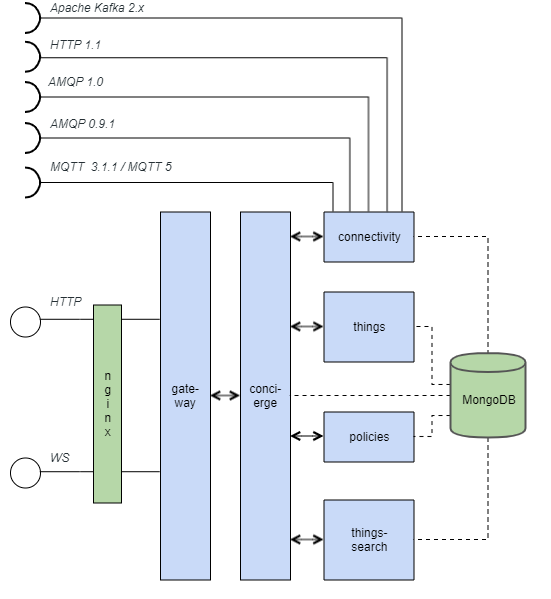
\includegraphics[width=0.8\linewidth]{img/ditto_arch.png}
    \caption[Aufbau eines Digital Twin Providers]{Aufbau eines Digital Twin Providers am Beispiel von Eclipse Ditto.\\Quelle:}
    \label{fig:ditto_arch}
\end{figure}

\subsection*{Integration von Strukturinformationen}
Eine der wichtigsten Funktionen des Digital Twin Providers stellt die strukturierte Bereitstellung der gesammelten Telemetriedaten dar. Da digitale Zwillinge nicht zwingend dem zugrundeligenden physischen Sensor entsprechen, sondern auf beliebige Art und Weise erweitert werden können, sind Strukturinformationen von elementarer Bedeutung, um den Nutzen zu erhöhen. Die Integration dieser Informationen muss optional sein, da sonst Einstiegshürden geschaffen werden, welche die \enquote{time to market} einer zu entwickelnden Applikation negativ beeinflussen können. Daher bietet es sich an eine extra Komponente in der Gesamtarchitektur bereitzustellen, welche optional hinzugefügt und integriert werden kann.

\begin{figure}
    \centering
    \begin{tikzpicture}[node distance=4cm]
        \node (device) [io] {Endgerät};
        \node (dr) [process, right of=device, xshift=2cm] {Device Registry};
        \node (dts) [process, below of=dr] {Digital Twin Provider};
        \node (vorto) [process, right of=dts] {Strukturregistry};
        \node (connector) [process, fill=green!30, right of=dr, yshift=-1.75cm] {Connector};
        \node (app) [startstop, below of=device] {Business Application};
    
        \draw [arrow] (device) -- (dr);
        \draw [arrow] (dr) -- (dts);
        \draw [arrow] (app) -- (dts);
    
        \draw [thick, dashed, color=red] (connector) -- (dr);
        \draw [thick, dashed, color=red] (connector) -- (dts);
        \draw [dashed] (connector) -| (device);
        \draw [dashed, thick] (vorto) -- (dts);
    \end{tikzpicture}
    \caption[Integration der Strukturregistry in die Gesamtarchitektur]{Integration der Strukturregistry in die Gesamtarchitektur.\\Quelle: Eigene Darstellung}
\end{figure}

Das einfügen einer Strukturregistry ermöglicht es, die Komplexität verschiedener Austauschformate zu reduzieren. Mithilfe einer Mapping-Engine, können Regeln definiert werden, die ein Eingangsformat in ein einheitliches Format zur Nutzung innerhalb einer Applikation transfomieren. Dies hat den Vorteil, die Kopplung zwischen Endgerät, dem korrespondierenden \ac{DT} und der Applikation zu verringern. Die nötige Logik, um die verschiedenen Datenformate zu interpretieren wird von der Strukturregistry übernommen und muss nicht in jeder konsumierenden Applikation umgesetzt werden.

Des weiteren können so ohne Anpassungen in einer Applikation vornehmen zu müssen weitere Gerätetypen genutzt werden. Selbst wenn sich die komplette Sensorenlandschaft ändert, z.B. bei einem Anbieterwechsel, o.ä., kann mithilfe eines Mappings innerhalb der Strukturregistry sichergestellt werden, dass das neue Datenformat in das einheitliche, von allen Applikationen verstandene Format transformiert wird.

Zusammenfassend lassen sich folgende Vorteile mit der Nutzung einer Strukturregistry erreichen:

\begin{enumerate}
    \item Die time to market wird reduziert, da Entwicklungsaufwände sinken und durch klare Datenformate parallelisiert werden können.
    \item Wartungsarbeiten oder spätere Anpassungen auf neue Anforderungen sind einfacher umsetzbar, da einheitliche Datenformate vorhanden sind.
\end{enumerate}

Sollte es nicht möglich sein, eine unabhängige Strukturregistry bereitzustellen, können diese Vorteile trotzdem erreicht werden. Dafür muss der Digital Twin Provider eine Mapping Engine anbieten, die es ermöglicht Telemetriedaten, die von der Device Registry empfangen werden, zu transformieren. So kann auch ohne den Einsatz einer dedizierten Strukturregistry der Vorteil einer einheitlichen Datenstruktur erreicht werden.\\
Ein Nachteil dieser leichtgewichten Variante ist jedoch, dass die Kopplung zwischen Digital Twin Provider und Device Registry noch einmal erhöht wird, was die Modularität der Architektur negativ beeinflusst.

\subsection{Verwaltung von digitalen Zwillingen}

Ein weiterer wichtiger Aspekt ist die Verwaltung digitaler Zwillinge. Der Digital Twin Provider erhält die Telemetriedaten über die Device Registry. Es gilt aber zusätzlich statische Informationen über den \ac{DT} zu verwalten. Dafür müssen entsprechende API Schnittstellen bereitgestellt werden.

Auch wird eine erweiterte Suchfunktionalität benötigt, um spezielle Gruppen digitaler Zwillinge einfach identifizieren zu können. Dies ermöglicht applikationspezifische Logik mithilfe von Suchanfragen umzusetzen. Ein exemplarische Aufbau eines digitalen Zwillings innerhalb eines Digital Twin Providers kann folgendermaßen aussehen:

\begin{verbatim}
{
  "thingId": "the.namespace:theId",
  "policyId": "the.namespace:thePolicyId",
  "definition": "org.eclipse.ditto:HeatingDevice:2.1.0",
  "attributes": {
      "someAttr": 32,
      "manufacturer": "ACME corp"
  },
  "features": {
      "heating-no1": {
          "properties": {
              "connected": true,
              "complexProperty": {
                  "street": "my street",
                  "house no": 42
              }
          },
          "desiredProperties": {
              "connected": false
          }
      },
      "switchable": {
          "definition": [ "org.eclipse.ditto:Switcher:1.0.0" ],
          "properties": {
              "on": true,
              "lastToggled": "2020-11-15T18:21Z"
          }
      }
  }
}
\end{verbatim}

Innerhalb der Struktur lassen sich einige umgesetzte Anforderungen erkennen. Eine Anforderung, welche bereits in der Device Registry eine große Rolle spielte, war eine Umsetzung eines Namespacing Konzepts. Dieses Konzept wird in dem Digital Twin provider mithilfe fester Präfixe erreicht. Exemplarisch dafür kann die \texttt{thingId} betrachtet werden. Der Namespace wird dabei mittels eines Doppelpunktes von dem eigentlichen \enquote{Namen} des \ac{DT}s abgetrennt. \\
Dieses Konzept kann auch bei anderen Ressourcen des Digital Twin Providers genutzt werden. Somit wird erreicht, dass der Provider von mehreren Anwendern gleichzeitig genutzt werden kann.

Des weiteren lässt sich die Persistenz der dynamischen und statischen Daten erkennen. Innerhalb der \texttt{attributes} sind alle statischen Informationen über den digitalen Zwilling gespeichert. Hierbei ist prinzipiell keine feste Struktur vorgegeben und es können beliebe Werte gespeichert werden. Diese Werte können zur weiteren Identifikation genutzt werden. Gleichzeitig können diese Werte bei der Suche und Gruppierung von digitalen Zwillingen eingesetzt werden.

\subsection{Integration von Policies zur Zugriffsbeschränkung}

Wie bereits in der Datenstruktur zu erkennen ist, muss dem digitalen Zwilling eine Policy zugewiesen werden. Die Aufgabe einer Policy besteht darin, Zugriffe auf Attribute oder den gesamten digitalen Zwilling zu steuern. So kann sichergestellt werden, dass Informationen nur berechtigten Applikationen zur Verfügung gestellt werden. Die Struktur einer Policy kann folgendermaßen aussehen:

\begin{verbatim}
{
  "policyId": "my.namespace:policy-a",
  "entries": {
    "observer": {
      "subjects": {
        "nginx:observer-client": {
          "type": "technical client"
        },
        "nginx:some-users": {
          "type": "a group of users"
        }
      },
      "resources": {
        "thing:/features/featureX": {
          "grant": ["READ"],
          "revoke": []
        },
        "thing:/features/featureY": {
          "grant": ["READ"],
          "revoke": []
        }
      }
    }
  }
}
\end{verbatim}

Die Umsetzung eines policy-basierten Zugriffssystems muss eine möglichst hohe Dynamik haben, damit die dynamische Struktur der Daten eines digitalen Zwillings unterstützt werden kann. Es lässt sich ausserdem erkenne, dass auch hier bei der \texttt{policyId} wieder dasselbe Konzept zum Namespacing genutzt wird, wie auch bei der Speicherung des \ac{DT}s an sich. Es können verschiedene \enquote{Rollen} innerhalb der Policy definert werden, welche unterschiedliche Nutzergruppen repräsentieren können. Grundsätzlich folgt die Implementierung aber dem Konzept einer \ac{ACL}. Es werden also \textbf{explizit} alle Nutzer benannt, die Zugriff auf eine Ressource haben. Diese werden innerhalb des \texttt{subject} Keys definiert. Die \texttt{resources} beschreiben ebenfalls \textbf{explizit} welche Operationen genehmigt oder verweigert

\begin{itemize}
    \item Bild über den internen Aufbau von Ditto
    \item Genauer auf problematische Funktionen eingehen, die in den Anforderungen beschrieben wurden
    \item Wo greift alles gut ineinander
    \item Tatsächliche Überleitung auf Softwareumsetzung
\end{itemize}

\large{Softwarekonzept}
\normalsize
\begin{itemize}
    \item Hono als DR
    \item Ditto als DT Provider
    \item Vorto als Strukturrepository
    \item \enquote{Am Beispiel eines Sensors mit LoRaWAN und TTN}
    \item Beschreiben der Schritte innerhalb der Umsetzung (Go-App)
    \item 
\end{itemize}

\large{Deployment}
\normalsize
\begin{itemize}
    \item Deplomyent via Container (Docker)
    \item verschiedene Methoden der Containerorchestrierung (docker-compose, kubernetes)
    \item Hinzufügen von Hard- und Softwaremonitoring
\end{itemize}
